\documentclass{article}
\usepackage[utf8]{inputenc}
\usepackage{graphicx}


\begin{document}
\title{Project Computer Graphics: OpenGl}
\author{Wald Habets \& Ruben Ballet}
\maketitle

\section{Inleiding}
\par
Dit bestand bevat het verslag van het project OpenGL, door Wald Habets en Ruben Ballet, voor het vak Computer Graphics. Dit verslag bespreekt de gemaakte keuzen betreffende datastructuren, file formaat en ontwerp van het project.

\section{Vereisten}

Deze sectie bespreekt de implementatie van de vereisten samen met de hierbij nodigge toelichting.

\paragraph{Weergave van een 3D omgeving}Als 3D omgeving de eerste wereld van het spel Mario64 gekozen.

\paragraph{Display Lists}Alle objecten worden in de wereld geïnstantiëerd met behulp van display lists, ook de objecten die maar één maal geïnstantiëerd moeten worden. Er is voor deze aanpak gekozen omwille van de manier waarop objecten worden ingeladen in het programma. Door display lists te gebruiken voor alle objecten, kunnen deze objecten worden ingeladen op een uniforme manier. Bij het inladen hoeven we ons dus geen zorgen te maken of een object slechts eenmalig of meerdere keren voorkomt.
\par
Het aanmaken van een display list gebeurt op dezelfde manier als besproken in de cursus (via glNewList, glBegin(GL\_TRIANGLES) en glCallList). De elementen die voor elk object worden opgenomen in de displaylist zijn de vertices met voor elke vertex de bijhorende normaal en texture-coördinaat. Transformaties worden niet opgenomen in de display list, zodat op deze manier elke instantie van een object zijn eigen positie, grootte en rotatie kan hebben.

\paragraph{File Formaat \& Hiërarchische relaties}Alle objecten zijn .obj-bestanden die worden ingeladen met behulp van de Assimp-library. Welke objecten moeten worden ingeladen, hun textures, positie, rotatie, schalering en onderlinge relatie wordt beschreven in een .json-bestand. Bij het opstarten van het programma wordt dit bestand ingelezen en op basis hiervan wordt de wereld gegenereerd.
\par
Er is gekozen om een bestand te gebruiken dan de volledige wereld beschrijft omdat dit ons toestaat de wereld makkelijk aan te passen zonder dat het nodig is om het programma opniew te compileren.
\par
Dit json-bestand houdt 4 lijsten bij: 
\begin{itemize}
	\item Een lijst van models: dit zijn alle .obj-bestanden die moeten worden geladen. (in het programma vertaald dit zich naar een display list).
	\item Een lijst van textures: dit zijn alle texture-bestanden die moeten worden geladen.
	\item Een lijst van groupen: dit is een verzameling entities. Elke group heeft een positie, rotatie en grootte.
	\item Een lijst van entities: dit zijn de objecten in de wereld. Elke entity heeft een model ID (de display list), een texture ID, een positie, rotatie en grootte en eventueel een group ID. Indien de entity tot een group behoort beschrijven positie, rotatie en grootte hun respectievelijke attributen binnen de group.
\end{itemize}
\par Voor de relatie tussen de klassen verwijzen we naar \textit{Afbeelding 1}.

\begin{figure}[!ht]
		\begin{minipage}[b]{1\linewidth}
			\centering
			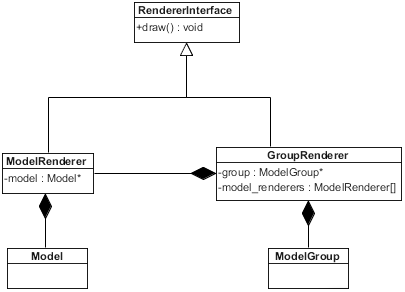
\includegraphics[width=0.7\linewidth]{relatie.png}
			\caption{Afbeelding 1}
		    \vspace{4ex}
		\end{minipage}
\end{figure}

\paragraph{Textures}Aan alle objecten kan een texture toegekend worden. Het binden van een texture gebeurt niet in de display list, waardoor een object dat meermaals geïnstantiëerd wordt verschillende textures kan hebben voor zijn verschillende instanties. Het is echter wel zo dat elke instantie ten hoogste één texture kan hebben.
\par
Het aanmaken en binden van textures gebeurt op dezelfde manier als besproken in de cursus (via glGenTextures, glBindTexture, etc). Voor het inladen van de afbeelding is voor de SOIL-library gekozen.

\paragraph{Visualisaties}Het programma ondersteunt de vereiste visualisaties: nl. flat-shaded, smooth-shaded, wire-frame (en non-wire-frame). De visualisatie kan worden aangepast via het menu (esc \textgreater \space settings).

\paragraph{Navigatie}Het programma ondersteunt navigatie via de muis en het toetsenbord. De sneltoesten kunnen worden geraadpleegd via het menu. (esc \textgreater \space key-bindings).
\par
De camera bestaad uit 3 klassen: één die de positie en rotatie omvat, één die de input van het toetsenbord afhandelt en één die de input van de muis afhandelt.
\par
De camera zelf bestaat houdt 2 punten en 4 vectoren bij, waarop alle manipulaties gebeuren. Deze 2 punten zijn de positie en het punt waar naar gekeken wordt. De 4 vectoren zijn:
\begin{itemize}
	\item een forward-vector die altijd naar voor is gericht (t.o.v. de camera, evenwijdig met xz)
	\item een right-vector die altijd naar rechts is gericht (t.o.v. de camera, evenwijdig met xz)
	\item een up-vector die altijd naar boven is gericht (evenwijdig met y)
	\item een looks-at-vector die de kijkhoek beschrijft (boven onder)
\end{itemize}
Het gebruik van deze 4 vectoren staat ons toe om alle mogelijke bewegingen op een snelle en uniforme manier te berekenen via matrix transformaties. Elke vector heeft namelijk zijn eigen translatie-, rotatie- en schalerings-functies. Streven van de camera gebeurt namelijk volgens de forward-, right- en up-vectoren en roteren gebeurt door de looks-at-vector te roteren rond deze vectoren.

\paragraph{Lichtbronnen}Het programma bevat 2 lichtbronnen, één vast in de wereld en één gemonteerd op de camera. De gemonteerde lichtbron wordt beschreven door de klasse \textit{Headlamp}. Ook de lichtbronnen volgen het model van de cursus (glEnable, glDisable en glLightfv).
\paragraph{Picking}

\end{document}